\section{Neural Networks}

\subsection{Deep Learning}

The concepts of deep learning studied in this section is going to be based on the work of \citet{goodfellow2016}.

There are several definitions of \gls*{ai} \citep{winston1992}, but the  computer scientist \citet{mccarthy2007} defines it as ``the science and engineering of making intelligent machines, especially intelligent computer programs.''.
He also states that ``it is related to the similar task of using computers to understand human intelligence, but AI does not have to confine itself to methods that are biologically observable.''.

The big area of study is the \gls*{ai} and it includes several branches like fuzzy logics, robotics, machine learning and so on. 
The later one, in turn, is another field with also some branches and one of them is the deep learning.
This can be represented in a Venn diagram, as the \cref{fig:venn_dl} shows.
However, all the three terms can be interchangeable in the major context.

\begin{figure}[H]
    \centering
    
\includegraphics{figures/2methodology/nn/venn_dl.pdf}
    \caption{Subareas of Artificial Intelligence}
    \label{fig:venn_dl}
\end{figure}

The deep learning history goes back to the 1940s and it had several names over the years. It was called by \emph{cybernetics} (1940s--1960s), \emph{connectionism} (1980s--1990s), and from 2006 until now is known as \emph{deep learning}.
The \gls*{dl} models were engineered systems inspired by the biological brain and they were denominated \gls*{ann}.
One of the motivations of the neural perspective was to understand that the brain provides a proof by example that intelligent behavior is possible and try to reverse engineer the computation principals behind the brain, duplicating its functionality.

\gls*{dl} today goes beyond the neuroscientist perspective and it is more of general principle of learning multiple levels of composition.

\subsection{Multilayer Perceptron}

A \gls*{mlp}, also known as \emph{deep network}, is the essence of \gls*{dl}. Basically, it is a mathematical function, formed by composing many simpler functions, mapping some set of input values to output values.
%
\begin{figure}[H]
    \centering
    \includegraphics{figures/2methodology/nn/mlp.pdf}
    \caption[Multilayer Perceptron Scheme]{Multilayer Perceptron Scheme. It resembles a human neuron: input layer data is equivalent to the dendrites; hidden layers are the equivalent of the axons; and the output layer are the equivalent of the nerve ending. The figure show two hidden layers, but it can contain multiple of them.}
\end{figure}

\noindent\textcolor{red}{PUT THE FORMULAS OF HOW MLP WORKS.}